\input{wsc14style.tex}     % download from author kit.  Style files for wsc formatting. Don't remove this line - required for generating the final paper!

\documentclass{wscpaperproc}
\usepackage{latexsym}
%\usepackage{caption}
\usepackage{graphicx}
\usepackage{mathptmx}
\usepackage{caption}
\usepackage{subcaption}
\usepackage{pgfplots}
\usetikzlibrary{patterns}
\usepackage{tikz}
\usepackage{multirow}

%
%****************************************************************************s
% AUTHOR: You may want to use some of these packages. (Optional)
\usepackage{amsmath}
\usepackage{amsfonts}
\usepackage{amssymb}
\usepackage{amsbsy}
\usepackage{amsthm}
\usepackage{algorithm}
\usepackage{gensymb}
\usepackage[noend]{algpseudocode}
\makeatletter
\def\BState{\State\hskip-\ALG@thistlm}
\makeatother
%****************************************************************************



%
%****************************************************************************
% AUTHOR: If you do not wish to use hyperlinks, then just comment
% out the hyperref usepackage commands below.

%% This version of the command is used if you use pdflatex. In this case you
%% cannot use ps or eps files for graphics, but pdf, jpeg, png etc are fine.

\usepackage[pdftex,colorlinks=true,urlcolor=blue,citecolor=black,anchorcolor=black,linkcolor=black]{hyperref}

%% The next versions of the hyperref command are used if you adopt the
%% outdated latex-dvips-ps2pdf route in generating your pdf file. In
%% this case you can use ps or eps files for graphics, but not pdf, jpeg, png etc.
%% However, the final pdf file should embed all fonts required which means that you have to use file
%% formats which can embed fonts. Please note that the final PDF file will not be generated on your computer!
%% If you are using WinEdt or PCTeX, then use the following. If you are using
%% Y&Y TeX then replace "dvips" with "dvipsone"

%%\usepackage[dvips,colorlinks=true,urlcolor=blue,citecolor=black,%
%% anchorcolor=black,linkcolor=black]{hyperref}
%****************************************************************************



		



%
%****************************************************************************
%*
%* AUTHOR: YOUR CALL!  Document-specific macros can come here.
%*
%****************************************************************************

% If you use theoremes
\newtheoremstyle{wsc}% hnamei
{3pt}% hSpace abovei
{3pt}% hSpace belowi
{}% hBody fonti
{}% hIndent amounti1
{\bf}% hTheorem head fontbf
{}% hPunctuation after theorem headi
{.5em}% hSpace after theorem headi2
{}% hTheorem head spec (can be left empty, meaning `normal')i

\theoremstyle{wsc}
\newtheorem{theorem}{Theorem}
\renewcommand{\thetheorem}{ \arabic{theorem}}
\newtheorem{corollary}[theorem]{Corollary}
\renewcommand{\thecorollary}{\arabic{corollary}}
\newtheorem{definition}{Definition}
\renewcommand{\thedefinition}{\arabic{definition}}


%#########################################################
%*
%*  The Document.
%*
\begin{document}

%***************************************************************************
% AUTHOR: AUTHOR NAMES GO HERE
% FORMAT AUTHORS NAMES Like: Author1, Author2 and Author3 (last names)
%
%		You need to change the author listing below!
%               Please list ALL authors using last name only, separate by a comma except
%               for the last author, separate with "and"
%
\WSCpagesetup{Sunderrajan, Aydt, Cai and Knoll}

% AUTHOR: Enter the title, all letters in upper case
\title{MAP STREAM: INITIALIZING WHAT-IF ANALYSES FOR REAL-TIME SYMBIOTIC TRAFFIC SIMULATIONS}

% AUTHOR: Enter the authors of the article, see end of the example document for further examples
\author{Abhinav Sunderrajan\\ [12pt]
TUM CREATE Ltd\\
1 CREATE Way\\
138602, SINGAPORE\\
% Multiple authors are entered as follows.
% You may also need to adjust the titlevbox size in the preamble - search for titlevboxsize
\and
Heiko Aydt \\[12pt]
TUM CREATE Ltd\\
1 CREATE Way \\
138602, SINGAPORE \\
\and
Wentong Cai\\ [12pt]
School of Computer Engineering\\
Nanyang Technological University\\
Nanyang Avenue 639798, SINGAPORE\\
\and
Alois Knoll\\ [12pt]
Robotics and Embedded Systems Group \\
Department of Informatics\\
Technische Universit\"at M\"unchen\\
Boltzmannstra{\ss}e 3\\
D-85748 Garching bei M\"unchen, GERMANY
}






\maketitle

\section*{ABSTRACT}
In the context of a city-scale symbiotic  traffic simulation, real-time data about the location of many vehicles are obtained in the form of a continuous data-stream. In this paper, we present a scalable solution for performing map-matching using sliding-windows over a GPS data-stream onto a digital road network for initializing the what-if analysis process involved in symbiotic simulations. We focus on the optimizations performed to ensure that the latency associated with the map-matching process is low while maintaining a high degree of accuracy. Experimental results reveal the range in terms of sampling interval and noise for acceptable reliability and latency.

\section{INTRODUCTION}
\label{sec:introduction}
Introduced in~\shortcite{fujimotoeditors}, symbiotic simulation is a paradigm which is characterized by a mutually beneficial relationship between the physical environment and the simulation system. While the simulation system benefits from the continuous measurements provided by the physical system, the latter benefits from the near real-time decisions provided by the former. Symbiotic simulations involve a what-if analysis (WIA) process which is responsible for creating and evaluating several alternative scenarios through simulations. Executing these simulations as fast as possible is important in the context of a symbiotic simulation. Initializing a simulation run with the state of the physical system is potentially time consuming. In this paper we present and evaluate an appropriate initialization method for traffic simulations.

As motivated in~\cite{aydt2012symbiotic}, a city-scale symbiotic traffic-simulation involving tens of thousands of vehicles depends on incorporating real-time measurements provided by white-box and gray-box vehicles which share information regarding their geo-location, speed and origin-destination (white-box vehicles only). For the symbiotic simulation to be effective, it is essential to process the data, initialize and execute the simulation with minimum latency. A symbiotic traffic-simulation could be initialized by using the GPS location information provided by the vehicles. However due to inaccuracies associated with GPS data~\shortcite{wang2011challenges} suitable  map-matching algorithms need to be employed. Map-matching refers to the process of aligning a sequence of GPS location data from a vehicle with a spatial road network to identify the road(s) the vehicle is traveling. Given the sheer number of vehicles on the entire road network of a city, the location of vehicles is obtained in the form of an unbounded, continuous data-stream. Hence traditional map-matching techniques which focus on matching over a batch of data are either unsuitable or need to be optimized. Given the streaming nature of the GPS probe data it is critical that the map-matching algorithm is not only reliable but also able to compute the results with minimal latency. In this paper we present and evaluate a scalable algorithm which can be used to map the position of several vehicles from a data-stream on to a digital road network using sliding windows. The solution also incorporates a set of optimizations in order to minimize the map-matching latency while maintaining a high degree of accuracy.

The organization of the rest of the paper is as follows. In Section~\ref{sec:map-matching-intro} we introduce the map-matching problem and discuss related work. In Section~\ref{sec:map-matching-stream} we present in detail our algorithm for map-matching over a data-stream while discussing the optimizations made for reducing the latency associated with map-matching. In Section~\ref{sec:evaluation} we present the results of our solution which compares two aspects of map matching namely GPS noise vs sampling interval vs reliability and GPS noise vs sampling interval vs latency. We present our conclusions in Section~\ref{sec:conclusion}. 


\section{MAP MATCHING PROBLEM}
\label{sec:map-matching-intro}

Map-matching algorithms have been used to map noisy GPS data on to a digital road network for supporting functions such as navigation in Intelligent Transportation Systems (ITS). Detailed review of existing map-matching techniques can be found in~\cite{quddus2007current}. Geometric map-matching algorithms~\cite{jagadeesh2004map} make use of the shape of the roads and (or) the trajectory of the vehicles on the roads. Topological map-matching~\cite{yin2004weight} algorithms consider the road connectivity and contiguity along with geometric features. Advanced techniques such as Kalman Filters~\cite{obradovic2006fusion}, have also been effectively used for map-matching.

Regardless of the approach of the approach they apply, all map-matching algorithms ultimately need to associate a GPS sample with a road. Due to inherent noise there is always some uncertainty with associating a GPS sample with a road. For example consider the case illustrated in Figure~\ref{fig:example}. The GPS sample $z_{1}$ could be associated with any of the three roads $\{AB, CD, EF\}$. Given a single geo-location, it is hard to identify the exact road segment a vehicle is on. Hence to make a guess on the probable road segment traversed, we need at least two signals from a single vehicle. Thus the second noisy signal $z_{2}$ and the associated roads $\{AB, CD\}$ are required.


\begin{figure}[h]
 \centering
 \includegraphics[scale=0.7]{hmm1.pdf}
 \caption{Example for uncertainty associated with map-matching.}
 \label{fig:example}
\end{figure}

We use a Hidden Markov Model(HMM) based algorithm for map matching. HMM is used to model a  process with hidden states using the  observed states. It is assumed that the hidden states form a Markov Chain. An HMM is able to incorporate noisy data elegantly and has found applications in several domains~\cite{rabiner1989tutorial}. Figure~\ref{fig:trellis} shows the Trellis diagram of the HMM for map-matching. Given a road network $G(V,E)$, where $V$ is a set of all vertices and $E$ is a set of all edges, a hidden state of the HMM represents the actual position of a vehicle on an edge $e_{t} \in E$ at time $t$. We assume that the future location of a vehicle depends only on the current location thus making the vehicular movements a Markov process. $Z=(z_{t}|t=1~...~n)$ denotes the entire trajectory of the vehicle from its origin to destination.  The noisy GPS data point or the observed state of the HMM at time $t$ is represented by $z_{t} \in Z$. Each $z_{t}$ is a tuple containing latitude, longitude, vehicle-id and time-stamp information as fields. Each edge $e_{t}$ is associated with a begin vertex $e_{t}.v_{begin}$ and an end vertex $e_{t}.v_{end}$. Finally for future reference, the term road segment refers to the sequence of edges constituting the shortest path from one vertex to another in the road network.

\begin{figure}[h]
 \centering
 \includegraphics[scale=0.5]{hmm_trellis.pdf}
 \caption{Trellis diagram for HMM.}
 \label{fig:trellis}
\end{figure}



The joint probability distribution of an HMM is given by Equation~\ref{eq:hmm_jpd}. The quantity $p(z_{1}|e_{1})\times p(e_{1})$ represents the initial distribution and is assumed to be known. The unknown terms namely the transition and emission probabilities need to be computed. Emission probabilities $p(z_{t}|e_{t})$ represents the probability of a noisy GPS data point $z_{t}$ being associated with an edge $e_{t} \in E$. Transition probabilities, $p(e_{t}|e_{t-1})$, represent the probability that a vehicle travels to edge $e_{t}$ given that it is currently on $e_{t-1}$.
\begin{equation} \label{eq:hmm_jpd}
p(z_{1},z_{2},z_{3}~ ... ~z_{n}, e_{1},e_{2},e_{3}~ ... ~e_{n} ) = p(z_{1}|e_{1})\times p(e_{1})\sum_{t=2}^n p(e_{t}|e_{t-1})\times p(z_{t}|e_{t})
\end{equation}



HMM has been used for map-matching in various other works including~\shortcite{newson2009hidden},~\cite{krumm2007map},~\shortcite{goh2012online}. The work done in~\cite{krumm2007map} and~\shortcite{newson2009hidden} (an enhancement of the former) treat map-matching as a batch problem and use the entire trajectory for computing the results. However we use the work done in~\cite{newson2009hidden} as the foundation for computing emission and transition probabilities. The work by~\shortcite{goh2012online} is close to our work since it focuses on keeping the latency associated with map-matching minimal while maintaining a high degree of accuracy for real time applications. For computing the transition probabilities,~\shortcite{goh2012online} train a Support Vector Machine classifier to classify incorrect and correct transitions from a given edge $e_{i}$ to edge $e_{j}$. The associated scoring functions of the classifier make use of the velocity information of the vehicle. Further they use sliding-windows of variable length (with an upper bound) before emitting the optimal results. In our work we fix the length of the sliding window used to two. While the accuracy of the algorithm can be expected to be lower, the latency for computing the results are much smaller. Further we also incorporate optimizations to reduce the latency for map-matching. Experiments were also performed to determine  the relative accuracy and time taken for map-matching under varying noise and sampling intervals $\delta$.

\section{MAP MATCHING OVER A DATA STREAM}
\label{sec:map-matching-stream}

\subsection{Map matching with sliding windows of size two}
\label{subsec:sliding-window}

 For implementing a real-time, on-line map-matching algorithm, the GPS signals belonging to a single vehicle are thus added to a sliding length window of size $2$. The  Trellis diagram shown in Figure~\ref{fig:trellis} thus reduces to computing only two states, i.e., $e_{t-1}$ to $e_{t}$ corresponding to $z_{t-1}$ to $z_{t}$. Consider an example where two successive, noisy GPS signals $z_{1},z_{2}$ could be associated with edges $e_{1}$ or $e_{2}$ and $e_{3}$ or $e_{4}$ respectively. The probability of the most likely route taken by the vehicle, $p_{route}$ based on Equation~\ref*{eq:hmm_jpd} is given by the maximum of the possible joint probability distributions which are calculated as shown in Equations~\ref{eq:hmm_Stream_1} to~\ref{eq:hmm_Stream_3}. As noted in Section~\ref{sec:map-matching-intro}, the unknown quantities namely the emission and transition probabilities need to be computed. 

\begin{equation} \label{eq:hmm_Stream_1}
p_{route}=max\Biggl(p(z_{1},z_{2},e_{1},e_{3}),p(z_{1},z_{2},e_{1},e_{4}),p(z_{1},z_{2},e_{2},e_{3}),p(z_{1},z_{2},e_{2},e_{4})\Biggr)
\end{equation}
Expanding the terms we get,
\begin{equation} \label{eq:hmm_Stream_2}
\begin{split}
p_{route}=max\Biggl((p(e_{1})\times p(z_{1}|e_{1})\times p(e_{3}|e_{1})\times p(z_{2}|e_{3})), (p(e_{1})\times p(z_{1}|e_{1})\times p(e_{4}|e_{1})\times p(z_{2}|e_{4})),\\ (p(e_{2})\times p(z_{1}|e_{2})\times p(e_{3}|e_{2})\times p(z_{2}|e_{3})), (p(e_{2})\times p(z_{1}|e_{2})\times p(e_{4}|e_{2})\times p(z_{2}|e_{4}))\Biggr)
\end{split}
\end{equation}
We now assume that $p(e_{t})$, i.e., the probability of a vehicle being on any of the roads in the proximity of the GPS sample is the same. Hence the above formula reduces to
\begin{equation} \label{eq:hmm_Stream_3}
\begin{split}
p_{route}=max\Biggl((p(z_{1}|e_{1})\times p(e_{3}|e_{1})\times p(z_{2}|e_{3})), (p(z_{1}|e_{1})\times p(e_{4}|e_{1})\times p(z_{2}|e_{4})),\\ (p(z_{1}|e_{2})\times p(e_{3}|e_{2})\times p(z_{2}|e_{3})), (p(z_{1}|e_{2})\times p(e_{4}|e_{2})\times p(z_{2}|e_{4}))\Biggr)
\end{split}
\end{equation}

Assuming a Gaussian noise~\cite{newson2009hidden} with standard deviation of $\sigma_{z}$ meters, the emission probabilities for each of the edges $e_{t}$ associated with a given GPS measurement $z_{t}$ are computed as follows
\begin{equation} 
\label{eq:emission_prob}
p(z_{t}|e_{t})= \frac{1}{\sigma_{z}\sqrt{2\pi}}\exp(-0.5(\frac{d_{p}(z_{t},e_{t})}{\sigma_{z}})^2)
\end{equation}
where $d_{p}(z_{t},e_{t})$ represents the perpendicular distance from the GPS sample $z_{t}$ to edge $e_{t}$.


\begin{figure}[h]
\label{fig:prob-density}
  \centering
\begin{minipage}[c]{.3\textwidth}
\centering
    \includegraphics[scale=0.25]{1sec.pdf}
    \caption*{$\delta=1 sec$}
\end{minipage}
\hspace*{\fill} % it's important not to leave blank lines before and after this command
\begin{minipage}[c]{.3\textwidth}
\centering
    \includegraphics[scale=0.25]{10sec.pdf}
    \caption*{$\delta=10 sec$}

\end{minipage}
\hspace*{\fill} % it's important not to leave blank lines before and after this command
\begin{minipage}[c]{.3\textwidth}
\centering
    \includegraphics[scale=0.25]{20sec.pdf}
    \caption*{$\delta=20 sec$}

\end{minipage}

\begin{minipage}[c]{.3\textwidth}
\centering
    \includegraphics[scale=0.25]{40sec.pdf}
    \caption*{$\delta=40 sec$}

\end{minipage}
\hspace*{\fill} % it's important not to leave blank lines before and after this command
\begin{minipage}[c]{.3\textwidth}
\centering
    \includegraphics[scale=0.25]{60sec.pdf}
    \caption*{$\delta=60 sec$}

\end{minipage}
\hspace*{\fill} % it's important not to leave blank lines before and after this command
\begin{minipage}[c]{.3\textwidth}
\centering
    \includegraphics[scale=0.25]{70sec.pdf}
    \caption*{$\delta=70 sec$}

\end{minipage}
 \caption{Probability density of $d_{t}$  at different sampling intervals}
\end{figure}


For computing the transition probabilities $p(e_{t}|e_{t-1})$, we make use of the previous work in ~\cite{newson2009hidden}. We compute the absolute value of the great circle distance between successive GPS samples from a vehicle and the route length traversed along road network graph $d_{t}$ as given by 
\begin{equation}
d_{t}=\mid gc(z_{t-1},z_{t})- routeLen(e_{t-1},e_{t})\mid
\end{equation}
The $routeLen$ function measures the length of the shortest path from vertex $e_{t-1}.v_{end}$ to the vertex $e_{t}.v_{begin}$. The $gc$ function computes the great circle distance between any two points on the earth using the haversine formula. Figure 3 shows the probability density of $d_{t}$ at different sampling intervals. The density as noted in ~\cite{newson2009hidden} fits an exponential distribution given by $p(d_{t})=\frac{1}{\beta}e^{\frac{-d_{t}}{\beta}}$. The parameter $\beta$ as suggested in ~\cite{newson2009hidden} is estimated as given in  Equation~\ref{eq:beta} where $D_{\delta}=(d_{t}|t=1 ... n)$ represents a set of $d_{t}$ for given a sampling frequency. The value for $\beta$ has been determined for different sampling intervals in order to ensure better and consistent estimates (represented as $\beta_{\delta}$). The concrete algorithm for a stream based map-matching using sliding window of size two is given in Algorithm~\ref{algo:map-matching-algo}.
\begin{equation}
\label{eq:beta}
\beta_{\delta}=\frac{1}{ln(2)}median(D_{\delta})
\end{equation}

\begin{algorithm}[h]
\caption{Map matching}
\label{algo:map-matching-algo}
{\bf Input: }
\begin{itemize}
\item $z_{1},z_{2}$ the two successive GPS samples from a single vehicle.
\item $G(V,E)$ the road network graph.
\item $\sigma_{z}$ standard deviation of GPS noise in meters.
\item $\beta_{\delta}$ the robust estimator for transition probabilities at the sampling interval $\delta$ .

\end{itemize}
{\bf Result: }Route from most probable edge $e_{1}\in E_{1}$ to most probable edge $e_{2}\in E_{2}$. Where $E_{1}$ and $E_{2}$ represent the set of edges in the proximity of $z_{1}$ and $z_{2}$ respectively.
\begin{algorithmic}[1]
\State $Mat_{rp}=\emptyset$
\State $Mat_{r}=\emptyset$
\State $E_{1}=$ Determine set of 8 closest edges to $z_{1}$

\State $E_{2}=$ Determine set of 8 closest edges to $z_{2}$


\For{$e_{1} \in E_{1}$}
	\State $p(e_{1}|z_{1}) = \frac{1}{\sigma_{z}\sqrt{2\pi}}\exp(-0.5(\frac{d_{p}(z_{1},e_{1})}{\sigma_{z}})^2)$
	\For{$e_{2} \in E_{2}$}
		\State $p(e_{2}|z_{2}) = \frac{1}{\sigma_{z}\sqrt{2\pi}}\exp(-0.5(\frac{d_{p}(z_{2},e_{2})}{\sigma_{z}})^2)$
		\State $d_{t} = \mid gc(z_{1},z_{2}) - routeLen(e_{1}.v_{end},e_{2}.v_{begin})\mid$
		\State $p(e_{2}|e_{1})=\frac{1}{\beta_{\delta}}e^\frac{-d_{t}}{\beta_{\delta}}$
		\State $Mat_{rp}[e_{1}][e_{2}]=p(e_{1}|z_{1})\times p(e_{2}|z_{2})\times p(e_{2}|e_{1})$
		\State $Mat_{r}[e_{1}][e_{2}]=shortestPath(e_{2}\gets e_{1})$
	\EndFor
	\EndFor
	
\State  $rowIndex,colIndex=argmax(Mat_{rp})$
\State {\bf return~}$Mat_{r}[rowIndex][colIndex]$
	
\end{algorithmic}
\end{algorithm}





\subsection{Optimizations for latency reduction}
\label{subsec:optimizations}
For rapid initialization of the symbiotic traffic simulation, we need to ensure that the latency associated with the map-matching algorithm is as low as possible. In this section we describe the steps taken for reducing latency for computing the emission and transition probabilities by partitioning the road network using QuadTrees.

\begin{figure}[h]
 \centering
 \includegraphics[scale=0.7]{QuadTree_partion.pdf}
 \caption{Road network of Singapore partitioned using QuadTrees}
 \label{fig:quadtree}
\end{figure}

Figure~\ref{fig:quadtree} shows the road network of Singapore partitioned using QuadTrees~\cite{finkel1974quad}. Note that Figure~\ref{fig:quadtree} shows only the leaf nodes of the QuadTree. A QuadTree is a hierarchical data-structure with each node having exactly four children.  QuadTrees are regularly used for partitioning two dimensional space for answering nearest neighbor queries efficiently. In comparison to a naive grid based partitioning, QuadTree partitioning takes into account the topology of the graph where denser regions are split into more regions in comparison to less dense regions. A node in the QuadTree is split into four equally sized children (or quadrants in the context of the 2 dimensional space) when the number of vertices in the node exceeds a predetermined limit. For the our road network containing roughly 44,000 vertices (and 88,000 edges) a node belonging to the QuadTree was split when the number of vertices associated with it exceeds 50.


Partitioning  the road network helps us to reduce the time required in finding the edges in the proximity of a GPS sample by limiting the search space to only those edges contained within the leaf node of the QuadTree into which the GPS sample falls. Of the edges belonging to a partition, the closest eight edges are chosen for evaluation. Further, partitioning the road network  helped us to speed up the process of evaluating the likely route alternatives for computing the transition probabilities for the HMM. For the shortest path computations used while estimating the transition probabilities, we used the arc-flag approach~\shortcite{mohring2007partitioning} to minimize the number of edges evaluated by the Dijkstra's algorithm. During the  initial preprocessing of the road network, we create an in-memory edge-partition(s) mapping. An edge is associated with a partition if it is part of  a shortest path leading to the partition. While computing the shortest paths from a vertex belonging to one partition to another vertex belonging to a different partition, only those edges leading to the destination partition are considered. This results in much faster shortest path computations. As detailed in~\shortcite{mohring2007partitioning}, the arc-flag approach lends itself perfectly for graphs partitioned using QuadTrees. 







\section{EVALUATION}
\label{sec:evaluation}

\subsection{Synthetic GPS data stream}

First and foremost a synthetic GPS data stream at different sampling intervals and with varying Gaussian noise was generated for performing the experimental analysis owing to the lack of vehicle trajectory data for Singapore. For generating a GPS stream at a given sampling frequency of $\delta$ seconds, we make use of the speed range information available for all edges constituting the road network. Given a speed range of $S_{i1} [\frac{m}{s}]$ to $S_{i2} [\frac{m}{s}]$ for an edge $e_{i}$, the distance traveled by the vehicle before emitting the next GPS location signal is taken to be $S_{i2}\times \delta$ meters. On reaching an edge $e_{j}$ with different values for $S_{j1}$ and $S_{j2}$ the distance traveled is updated accordingly as  $\delta \times S_{j2}$ meters. The steps are repeated for 50 randomly chosen routes at different sampling frequencies. Once the noise free GPS signals are created for 50 routes at different sampling frequencies, we add Gaussian noise of zero mean and varying standard deviation of $\sigma_{z}$ meters at random angle $\theta$ between 0$\degree$ and 360$\degree$ from the original location. Figure~\ref{fig:noise} shows a GPS signal shifted from its original location of $e_{1}$ to $z_{1}$ due to noise. 

\begin{figure}[!htbp]
 \centering
 \includegraphics[scale=0.8]{gaussian_noise.pdf}
 \caption{Shifted GPS position due to noise}
 \label{fig:noise}
\end{figure}



\subsection{Experimental results}
\label{subsec:exp-setup}

In this section we describe the sequence of steps used to evaluate the efficacy of the map-matching algorithm discussed in Section~\ref{sec:map-matching-stream}. We are concerned with two aspects of performance, namely the reliability and the latency when identifying the correct road segment the vehicle(s) is driving on. For measuring reliability, consider a case where a vehicle emits $n$ GPS signals from its origin to destination. The entire route then consists of $n-1$ segments. The chosen road segment thus represents the shortest path from the most probable edge $e_{t-1}$ associated with the GPS data-point $z_{t-1}$ to the most probable edge $e_{t}$ associated with $z_{t}$. Hence reliability measures the percentage of correctly mapped segments along the entire route. Figure~\ref{fig:reliability} shows the reliability of the algorithm under varying sampling intervals when the standard deviation of Gaussian noise increases. For the evaluation, the number of routes considered was 50 and the results were averaged over 10 repetitions.

\begin{figure}[h]
 \centering
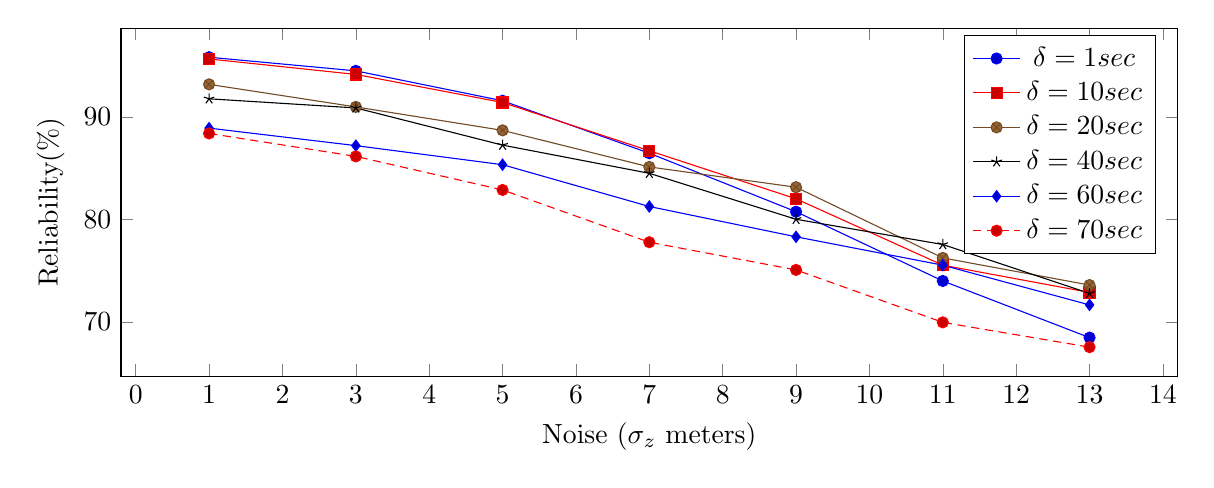
\begin{tikzpicture}
\begin{axis}[width=15.0cm,height=6.0cm,
	xlabel={Noise ($\sigma_{z}$ meters)},
	ylabel={Reliability(\%)}
]
\addplot coordinates {
	(1,95.83)    (3,94.50)   (5,91.58)
	(7,86.46)  (9,80.75)  (11,73.99)
	(13,68.46) 
};

\addplot coordinates {
	(1,95.66)    (3,94.15)   (5,91.41)
	(7,86.70)  (9,82.01)  (11,75.53)
	(13,72.87) 
};

\addplot coordinates {
	(1,93.18)    (3,90.98)   (5,88.69)
	(7,85.12)  (9,83.14)  (11,76.24)
	(13,73.59) 
};

\addplot coordinates {
	(1,91.77)    (3,90.88)   (5,87.25)
	(7,84.50)  (9,80.01)  (11,77.55)
	(13,72.78) 
};

\addplot coordinates {
	(1,88.91)    (3,87.20)   (5,85.34)
	(7,81.26)  (9,78.30)  (11,75.53)
	(13,71.65) 
};

\addplot coordinates {
	(1,88.39)    (3,86.15)   (5,82.875)
	(7,77.77)  (9,75.07)  (11,69.95)
	(13,67.53) 
};
\legend{$\delta=1 sec$,$\delta=10 sec$,$\delta=20 sec$,$\delta=40 sec$,$\delta=60 sec$,$\delta=70 sec$}
\end{axis}
\end{tikzpicture}
\caption{Noise vs sampling interval vs reliability}
 \label{fig:reliability}
\end{figure}



Computational latency measures the time interval between the arrival of the second GPS signal (two successive GPS signals are necessary to map the correct road segment the vehicle is traversing upon) and the time at which the algorithm emits the result of the matched road segment irrespective of the result correctness. Figure~\ref{fig:latency} shows the average latency values for matching a single segment under varying noise and sampling intervals. The results are once again averaged over 50 routes and 10 repetitions for a given sampling frequency and noise.

\begin{figure}[h]
 \centering
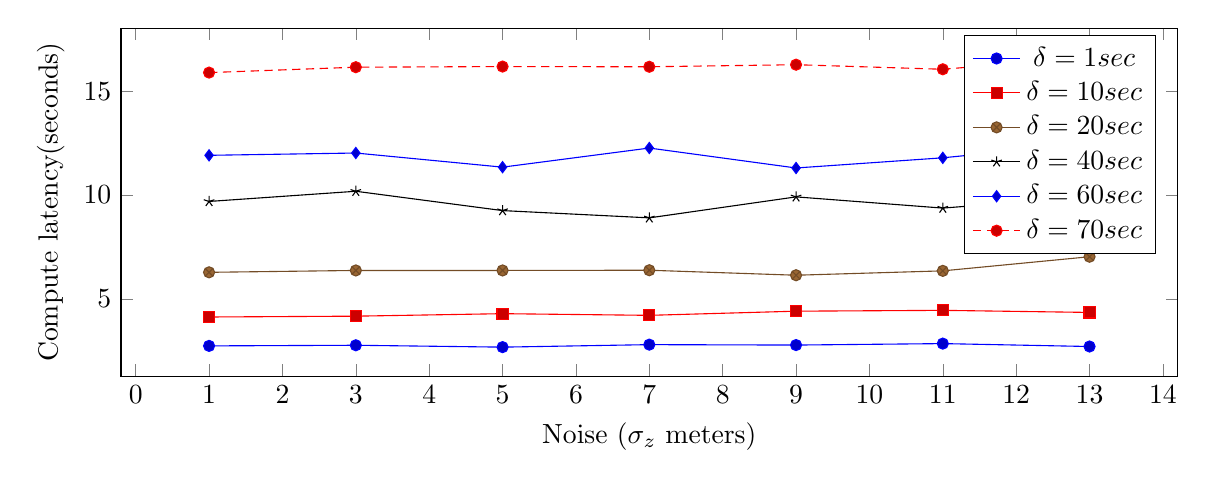
\begin{tikzpicture}
\begin{axis}[width=15.0cm,height=6.0cm,
	xlabel={Noise ($\sigma_{z}$ meters)},
	ylabel={Compute latency(seconds)}
]
\addplot coordinates {
	(1,2.74)    (3,2.77)   (5,2.68)
	(7,2.8)  (9,2.78)  (11,2.85)
	(13,2.71) 
};

\addplot coordinates {
	(1,4.13)    (3,4.17)   (5,4.29)
	(7,4.21)  (9,4.41)  (11,4.45)
	(13,4.35) 
};

\addplot coordinates {
	(1,6.28)    (3,6.37)   (5,6.37)
	(7,6.38)  (9,6.14)  (11,6.35)
	(13,7.03) 
};

\addplot coordinates {
	(1,9.69)    (3,10.18)   (5,9.25)
	(7,8.90)  (9,9.91)  (11,9.37)
	(13,9.92) 
};

\addplot coordinates {
	(1,11.91)    (3,12.02)   (5,11.34)
	(7,12.26)  (9,11.30)  (11,11.79)
	(13,12.49) 
};

\addplot coordinates {
	(1,15.89)    (3,16.15)   (5,16.18)
	(7,16.17)  (9,16.27)  (11,16.05)
	(13,16.63) 
};
\legend{$\delta=1 sec$,$\delta=10 sec$,$\delta=20 sec$,$\delta=40 sec$,$\delta=60 sec$,$\delta=70 sec$}
\end{axis}

\end{tikzpicture}
\caption{Noise vs sampling interval vs compute latency}
 \label{fig:latency}
\end{figure}




\subsection{Discussion of results}
\label{subsec:result-discuss}

 An example of the map-matching performed using the algorithm discussed in Section~\ref{sec:map-matching-stream} is illustrated in Figure~\ref{fig:complexity}. The interval between successive samples is 20 seconds with the Gaussian noise having a standard deviation of 11 meters 0 mean. Computing the emission and transmission probabilities results in the algorithm mapping GPS samples A and B to the incorrect road segment (marked in red) instead of the correct one marked in green. The error is corrected once the next GPS sample C is received. Note that the emission (and transition) probabilities  are computed once more for B  along with point C to identify the correct road segment. Not retaining the previous results thus enables the algorithm to recover from wrongly matched road segments. Finally we have not considered errors where the GPS signal gets mapped to a wrong partition due to noise. We propose to correct this error by considering multiple partitions if the point lies close to the boundary of two or more partitions as a part of future work.

\begin{figure}[!htbp]
 \centering
 \includegraphics[scale=0.58]{complexity.pdf}
 \caption{Source of errors while determining the path followed by the vehicle}
 \label{fig:complexity}
\end{figure} 

The second crucial aspect that needs discussion is that of computational latency. The results in Figure~\ref{fig:latency} indicate that the latency is noise invariant for a given sampling frequency. This is not surprising since the most probable segment is emitted without checking for result correctness. The latency increases as sampling frequency increases since the shortest path computations for transition probabilities are higher for vertices farther apart on the road network. Considering that we plan to implement a parallel version of the algorithm to match the position of several vehicles from a high velocity data-stream, it would be very useful to get a good idea about the latency. Given a scenario of 100,000 vehicles emitting GPS signals every second, despite the high degree of accuracy at low noise (Figure~\ref{fig:reliability}) it would be infeasible to implement the algorithm since the latency for map-matching exceeds 2 seconds resulting in 200,000 more records to be kept in memory even before we have the first segment for the vehicles mapped. For applications dealing with high velocity data-streams, large processing latencies could result in memory bottlenecks.

Considering a high degree of accuracy (even at reasonably high levels of noise) and less computational latency in comparison to the sampling intervals, GPS streams with $\delta=10$ seconds to $\delta=40$ seconds appear to be the most effective. For $\delta<10$ seconds, intermediate records can be filtered to achieve reasonable latency without compromising on accuracy.


\section{CONCLUSIONS AND FUTURE WORK}
\label{sec:conclusion}

In this paper we described and evaluated a map-matching algorithm which maps a GPS data-stream to a digital road network. We also implemented a couple of optimizations which reduce the latencies associated with computing the emission and transmission probabilities by using QuadTrees and a heuristic based on shortest path computations respectively.  The results indicate that the reliability was in the range of $85\% - 92\%$ when $\delta$ was in the range of 10 seconds to 40 seconds and standard deviation of noise was in the range of 5 meters to 9 meters. The aforementioned noise range is based on the data-analysis of large scale GPS probe data in ~\shortcite{wang2011challenges}. 

Though the experiments were performed and evaluated for the GPS data emitted by a single vehicle, we expect a parallel version of the algorithm to do the map-matching task over hundreds to thousands of vehicles to initialize a city-scale real-time symbiotic traffic simulation. As a part of future work, we plan to implement a parallel version of the presented algorithm using stream-processing engines such as STORM~\cite{STORM}. Finally from the perspective of a traffic simulation we plan to update the probability of vehicle taking an edge at a split on the road network (see Figure~\ref{fig:split}) based on historic information. The edge probabilities at splits can than be used to enhance the accuracy of the transition probabilities.
\begin{figure}[!htbp]
 \centering
 \includegraphics[scale=0.6]{split.pdf}
 \caption{Update probability of vehicle taking an edge at split based on count. }
 \label{fig:split}
\end{figure}


\section*{ACKNOWLEDGMENTS}
This work was financially supported by the Singapore National Research Foundation under its Campus for Research Excellence And Technological Enterprise (CREATE) programme.

% Please don't exchange the bibliographystyle style
\bibliographystyle{wsc}
% AUTHOR: Include your bib file here
\bibliography{demobib}
\newpage
\section*{AUTHOR BIOGRAPHIES}
\noindent {\bf ABHINAV SUNDERRAJAN} is a Research Associate at TUM CREATE Ltd., a company dedicated to research in all aspects of electro-mobility. He received his Masters in Computing from the National University of Singapore. His email address is \email{abhinav.sunderrajan@tum-create.edu.sg}.\\

\noindent {\bf HEIKO AYDT} received his Ph.D. degree in Computer Science from Nanyang Technological University (NTU), Singapore and his M.Sc. degree from the Royal Institute of Technology (KTH) in Stockholm. In 2006 he joined the Parallel and Distributed Computing Centre at NTU as Research Associate where he worked on several projects concerned with simulation-based optimisation and agent-based crowd simulation. In 2011, he joined TUM CREATE as Research Fellow and as of December 2012, he assumed the role of Principal Investigator for RP 5. His research at TUM CREATE is concerned with the analysis of the potential impact of electromobility on the infrastructure and the environment from a complex systems perspective. His current research interests are agent-based simulation, complex adaptive systems, symbiotic simulation, evolutionary computing and simulation-based optimisation. His email address is \email{heiko.aydt@tum-create.edu.sg}.\\

\noindent {\bf WENTONG CAI} is a Professor in the School of Computer Engineering at Nanyang Technological University, Singapore. He is also the Director of the Parallel and Distributed Computing Centre. His expertise is mainly in the areas of Modeling and Simulation (particularly, modeling and simulation of large-scale complex systems, and system support for distributed simulation and virtual environments) and Parallel and Distributed Computing (particularly, Cloud, Grid and Cluster computing). His web page is \hyperref{http://www.ntu.edu.sg/home/aswtcai/}{}{}{http://www.ntu.edu.sg/home/aswtcai/} and his email address is \email{aswtcai@ntu.edu.sg}.\\

\noindent {\bf ALOIS KNOLL} received his diploma (MSc) degree in Electrical/Communications Engineering from the University of Stuttgart and his PhD degree in Computer Science from the Technical University of Berlin. He served on the faculty of the computer science department of TU Berlin until 1993, when he qualified for teaching computer science at a university (habilitation). He then joined the Technical Faculty of the University of Bielefeld, where he was a full professor and the director of the research group Technical Informatics until 2001. Between May 2001 and April 2004 he was a member of the board of directors of the Fraunhofer-Institute for Autonomous Intelligent Systems. At AIS he was head of the research group "Robotics Construction Kits", dedicated to research and development in the area of educational robotics. Since autumn 2001 he has been a professor of Computer Science at the Computer Science Department
of the Technische Universit\"at M\"unchen. He is also on the board of directors of the Central Institute of Medical Technology at TUM (IMETUM-Garching); between April 2004 and March 2006 he was Executive Director of the Institute of Computer Science at TUM. His research interests include cognitive, medical
and sensor-based robotics, multi-agent systems, data fusion, adaptive systems and multimedia information retrieval. His email address is \email{knoll@in.tum.de}.




\end{document}

